\section{Experiments}

\subsection{Experimental Setup}

\textbf{Datasets.} To comprehensively evaluate AgeMem, we select five widely-used datasets in LLM-based agent research: ALFWorld~\citep{shridhar2020alfworld}, SciWorld~\citep{wang2022scienceworld}, PDDL~\citep{chang2024agentboard}, BabyAI~\citep{chevalier2018babyai}, and HotpotQA~\citep{yang2018hotpotqa}. These datasets cover embodied action, game-based reasoning, and knowledge-intensive question answering, providing diverse evaluation scenarios. Since the HotpotQA dataset contains both questions and supporting facts, automatically providing Stage~1 contextual information, AgeMem is fine-tuned with RL \textit{only on the HotpotQA training set} and then evaluated directly on all datasets. Detailed dataset statistics are provided in Appendix~\ref{app:datasets}.
\\
\textbf{Evaluation metrics.} For the primary task completion metrics, we adopt Success Rate (SR) for ALFWorld, SciWorld, and BabyAI, Progress Rate (PR) for PDDL, and LLM-as-a-Judge (J) for HotpotQA. Additionally, we employ an LLM-based evaluator to assess the quality of stored long-term memory during knowledge reasoning, measured by Memory Quality (MQ). The prompts of the LLM-based evaluation are provided in Appendix~\ref{app:evaluation}.
\\
\textbf{Baselines \& LLM backbones.} We compare AgeMem against four representative agent LTM systems: LangMem~\citep{langmem2025}, A-Mem~\citep{xu2025mem}, Mem0~\citep{chhikara2025mem0}, and $\text{Mem0}^g$ (a graph-based variant officially provided as part of Mem0). To better demonstrate the effectiveness of RL training, we also include AgeMem-noRL, which is not fine-tuned with RL. In ablation studies on STM, we compare STM tools with RAG approach. For the base agent models, we use Qwen2.5-7B-Instruct and Qwen3-4B-Instruct. More baseline configurations are in Appendix~\ref{app:baselines}.
\\
\textbf{Implementation details.} We build agents using the Agentscope framework~\citep{gao2025agentscope} and fine-tune AgeMem using the Trinity framework~\citep{pan2025trinity}. For all reward weights in the reward function, we use uniform coefficients of 1.0 without manual tuning. Further implementation details are provided in Appendix~\ref{app:implementation}.


\begin{table*}[t]
\centering
\small
\caption{Performance comparison across five benchmarks. The \textbf{best} and \underline{second-best} results are marked.}
\label{tab:main_results}
\setlength{\tabcolsep}{6pt}
\begin{tabular}{@{}l|l|@{\hspace{6pt}}ccccc@{\hspace{6pt}}|c@{}}
\toprule
\textbf{LLM Backbone} & \textbf{Method} & \textbf{ALFWorld} & \textbf{SciWorld} & \textbf{PDDL} & \textbf{BabyAI} & \textbf{HotpotQA} & \textbf{Average} \\
\midrule
\multirow{7}{*}{\textbf{Qwen2.5-7B-Instruct}} 
& No-Memory & 27.16 & 13.80 & 10.15 & 50.80 & 38.36 & 28.05 \\
& LangMem & \underline{38.27} & 28.29 & 15.85 & 51.34 & 37.43 & 34.23 \\
& A-Mem & 34.68 & 28.06 & \textbf{18.39} & 58.82 & 43.95 & 36.78 \\
& Mem0 & 37.49 & 26.99 & 13.96 & \underline{60.58} & \underline{46.66} & \underline{37.14} \\
& Mem0$^{g}$ & 35.34 & \underline{30.50} & 14.86 & 58.78 & 42.06 & 36.31 \\
% \cmidrule(lr){2-8}
& \cellcolor{gray!15}AgeMem-noRL & \cellcolor{gray!15}37.90 & \cellcolor{gray!15}28.67 & \cellcolor{gray!15}8.87 & \cellcolor{gray!15}46.34 & \cellcolor{gray!15}45.36 & \cellcolor{gray!15}33.43 \\
& \cellcolor{gray!15}AgeMem (Ours) & \cellcolor{gray!15}\textbf{41.07} & \cellcolor{gray!15}\textbf{35.55} & \cellcolor{gray!15}\underline{17.31} & \cellcolor{gray!15}\textbf{61.42} & \cellcolor{gray!15}\textbf{54.44} & \cellcolor{gray!15}\textbf{41.96} \\
\midrule
\multirow{7}{*}{\textbf{Qwen3-4B-Instruct}} 
& No-Memory & 38.51 & 47.89 & 30.14 & 55.83 & 47.48 & 43.97 \\
& LangMem & 40.89 & 50.42 & 28.42 & 53.80 & 42.70 & 43.25 \\
& A-Mem & 34.31 & 50.14 & \underline{34.41} & \underline{61.35} & 48.48 & \underline{45.74} \\
& Mem0 & \underline{41.17} & \underline{51.38} & 31.72 & 60.05 & 39.16 & 44.70\\
& Mem0$^{g}$ & 36.69 & 47.76 & 29.61 & 57.59 & 38.12 & 41.95 \\
% \cmidrule(lr){2-8}
& \cellcolor{gray!15}AgeMem-noRL & \cellcolor{gray!15}38.02 & \cellcolor{gray!15}50.42 & \cellcolor{gray!15}27.52 & \cellcolor{gray!15}57.48 & \cellcolor{gray!15}\underline{54.49} & \cellcolor{gray!15}45.59 \\
& \cellcolor{gray!15}AgeMem (Ours) & \cellcolor{gray!15}\textbf{48.97} & \cellcolor{gray!15}\textbf{59.48} & \cellcolor{gray!15}\textbf{35.07} & \cellcolor{gray!15}\textbf{72.56} & \cellcolor{gray!15}\textbf{55.49} & \cellcolor{gray!15}\textbf{54.31} \\
\bottomrule
\end{tabular}
\vspace{-0.3cm}
\end{table*}

\subsection{Main Results}
\textbf{Comparison with counterparts.} Table~\ref{tab:main_results} shows that AgeMem achieves the highest average performance on both Qwen2.5-7B-Instruct (41.96\%) and Qwen3-4B-Instruct (54.31\%), outperforming all baselines across five datasets with relative gains of 49.59\% and 23.52\% over no-memory, respectively. Compared to the best baselines (Mem0 and A-Mem), AgeMem improves by 4.82 and 8.57 percentage points on average. RL training contributes 8.53 percentage points and 8.72 percentage points improvements over AgeMem-noRL, validating the three-stage progressive RL strategy.
\begin{figure}[t]
\centering
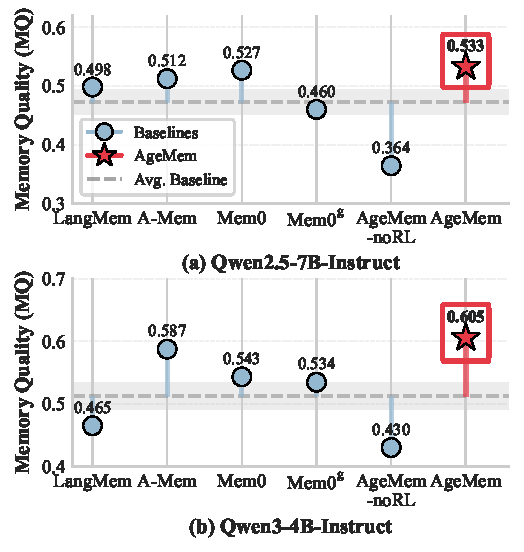
\includegraphics[width=0.4\textwidth]{results/fig_memory_quality.pdf}
\caption{Memory Quality scores for different methods on HotpotQA. Higher scores indicate better relevance between stored memories and ground-truth facts.}
\label{fig:memory_quality}
\end{figure}
\begin{figure}[t]
\centering
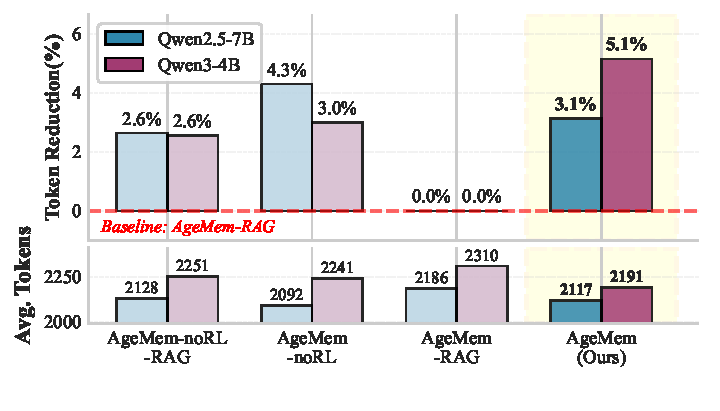
\includegraphics[width=0.48\textwidth]{results/fig_stm_management.pdf}
\caption{Average prompt token counts under different STM management configurations on HotpotQA. The suffix ``-RAG'' indicates the adoption of RAG in place of STM tool-based management.}
\label{fig:stm_management}
\end{figure}
\begin{table}[t]
\centering
\small
\caption{Tool usage statistics on HotpotQA. Numbers show average calls per episode.}
\label{tab:tool_usage}
% \resizebox{\columnwidth}{!}{%
\begin{tabular}{@{}l|cc|cc@{}}
\toprule
\multirow{2}{*}{\textbf{Tool Category}} & \multicolumn{2}{c|}{\textbf{Qwen2.5-7B}} & \multicolumn{2}{c}{\textbf{Qwen3-4B}} \\
\cmidrule(lr){2-3} \cmidrule(lr){4-5}
 & noRL & GRPO & noRL & GRPO \\
\midrule
\multicolumn{5}{c}{\textbf{\emph{LTM Tool Statistics}}} \\
\midrule
\textsc{Add} Memory & 0.92 & 1.64 & 2.49 & 2.64 \\
\textsc{Update} Memory & 0.00 & 0.13 & 0.13 & 0.34 \\
\textsc{Delete} Memory & 0.00 & 0.08 & 0.00 & 0.22 \\
\midrule
\multicolumn{5}{c}{\textbf{\emph{STM Tool Statistics}}} \\
\midrule
\textsc{Retrieve} Memory & 2.31 & 1.95 & 4.62 & 4.35 \\
\textsc{Summary} Context & 1.08 & 0.82 & 0.11 & 0.96 \\
\textsc{Filter} Context & 0.02 & 0.31 & 0.15 & 0.16 \\
\midrule
\textbf{Total Calls} & 4.33 & 4.92 & 7.50 & 8.67 \\
\bottomrule
\end{tabular}%
% }
\vspace{-0.3cm}
\end{table}
\\
\textbf{Quality of stored long-term memories.} To evaluate the quality of stored memories, we leverage the ground-truth facts provided in the HotpotQA dataset and assess the relevance between stored memories and these facts using an LLM-based evaluator. Figure~\ref{fig:memory_quality} presents the Memory Quality (MQ) scores for different baselines. AgeMem achieves the highest memory quality on both model backbones, with MQ scores of 0.533 and 0.605, respectively. This indicates that the unified memory management framework not only improves task performance but also promotes the storage of high-quality, reusable knowledge. The comparison with baseline methods further validates that AgeMem's tool-based memory operations lead to more selective and higher-quality memory construction.
\\
\textbf{Effectiveness of STM management.} We evaluate the effectiveness of STM management by measuring the prompt token count under different configurations on HotpotQA. Figure~\ref{fig:stm_management} shows that AgeMem successfully reduces prompt token usage compared to variants without STM tools (-RAG). On Qwen2.5-7B-Instruct, AgeMem uses 2,117 tokens on average, compared to 2,186 tokens for AgeMem-RAG, representing a reduction of 3.1\%. On Qwen3-4B-Instruct, the reduction is even more pronounced: AgeMem uses 2,191 tokens versus 2,310 tokens for AgeMem-RAG, a reduction of 5.1\%. These results demonstrate that the learned STM management tools effectively control context expansion, enabling more efficient token usage while maintaining task performance.
\begin{figure*}[t]
  \centering
  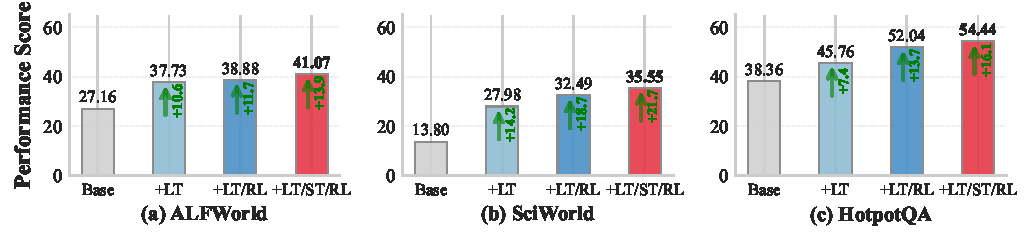
\includegraphics[width=0.9\textwidth]{results/fig_ablation_components.pdf}
  \caption{Ablation study on LTM, STM, and RL components (Qwen2.5-7B-Instruct). 
  \textbf{Base}: No-memory baseline; \textbf{+LT}: AgeMem-noRL-RAG (LTM tools only); 
  \textbf{+LT/RL}: AgeMem-RAG (RL with LTM tools); 
  \textbf{+LT/ST/RL}: AgeMem (full AgeMem system with RL). 
  Green arrows indicate performance gains over the baseline. }
  % Results for Qwen3-4B-Instruct are provided in Appendix~\ref{app:ablation}.}
  \label{fig:ablation_components}
\end{figure*}
\\
\textbf{Tool usage analysis.}
Table~\ref{tab:tool_usage} reports tool usage statistics before and after RL fine-tuning on HotpotQA. RL training substantially increases the use of long-term memory tools, especially \textsc{Add} and \textsc{Update}. On Qwen2.5-7B-Instruct, \textsc{Add} operations rise from 0.92 to 1.64, and \textsc{Update} operations appear after training (0.13 v.s.\ nearly zero). Similar trends are observed on Qwen3-4B-Instruct, with higher frequencies of both \textsc{Add} and \textsc{Update}.
For short-term memory tools, RL leads to more balanced tool usage. The frequency of \textsc{Filter} increases notably (e.g., from 0.02 to 0.31 on Qwen2.5), indicating proactive context control, while \textsc{Retrieve} remains relatively stable. Overall, these patterns suggest that RL training enables coordinated and adaptive memory management. Detailed case studies are provided in Appendix~\ref{app:case_study}.

\subsection{Ablation Studies}
\textbf{LTM-STM components.}
To validate the contributions of individual components, we conduct ablation studies on LTM, STM, and RL training. Figure~\ref{fig:ablation_components} presents results on three representative datasets using Qwen2.5-7B-Instruct as the backbone (results for Qwen3-4B-Instruct are provided in Appendix~\ref{app:ablation}).
Adding LTM alone (+LT) yields substantial gains of +10.6\%, +14.2\%, and +7.4\% over the baseline. Incorporating RL training (+LT/RL) further improves performance, particularly on HotpotQA (+6.3\%), demonstrating the effectiveness of our reward-based optimization. The full AgeMem system (+LT/ST/RL) achieves the best results across all benchmarks, with overall improvements of +13.9\%, +21.7\%, and +16.1\%. Notably, adding STM tools provides the most significant boost on SciWorld (+3.1\%) and HotpotQA (+2.4\%), validating that learned context management outperforms static RAG approaches. These progressive improvements confirm that unified memory management with end-to-end RL is essential for optimal agent performance.
\\
\textbf{Reward function.}
To demonstrate the effectiveness of our multi-component reward function design, we compare the full reward function (All-Returns) against a variant using only $R_{\text{task}}$ (Answer-Only).
Figure~\ref{fig:reward_convergence} shows the reward convergence curves of Qwen2.5-7B-Instruct during GRPO training on HotpotQA. The full reward function leads to significantly faster convergence and higher final performance compared to the task-only variant. As detailed in Table~\ref{tab:reward_ablation}, the All-Returns strategy achieves higher LLM-as-a-Judge scores (0.544 v.s. 0.509) while maintaining substantially better memory quality (0.533 v.s. 0.479).  Notably, despite using more tokens (2117 v.s. 2078), the All-Returns strategy achieves better overall performance, indicating that the additional context and memory operations contribute meaningfully to reasoning quality. Similar patterns are observed on Qwen3-4B-Instruct (see Appendix~\ref{app:qwen3_results}).

\begin{figure}[t]
\centering
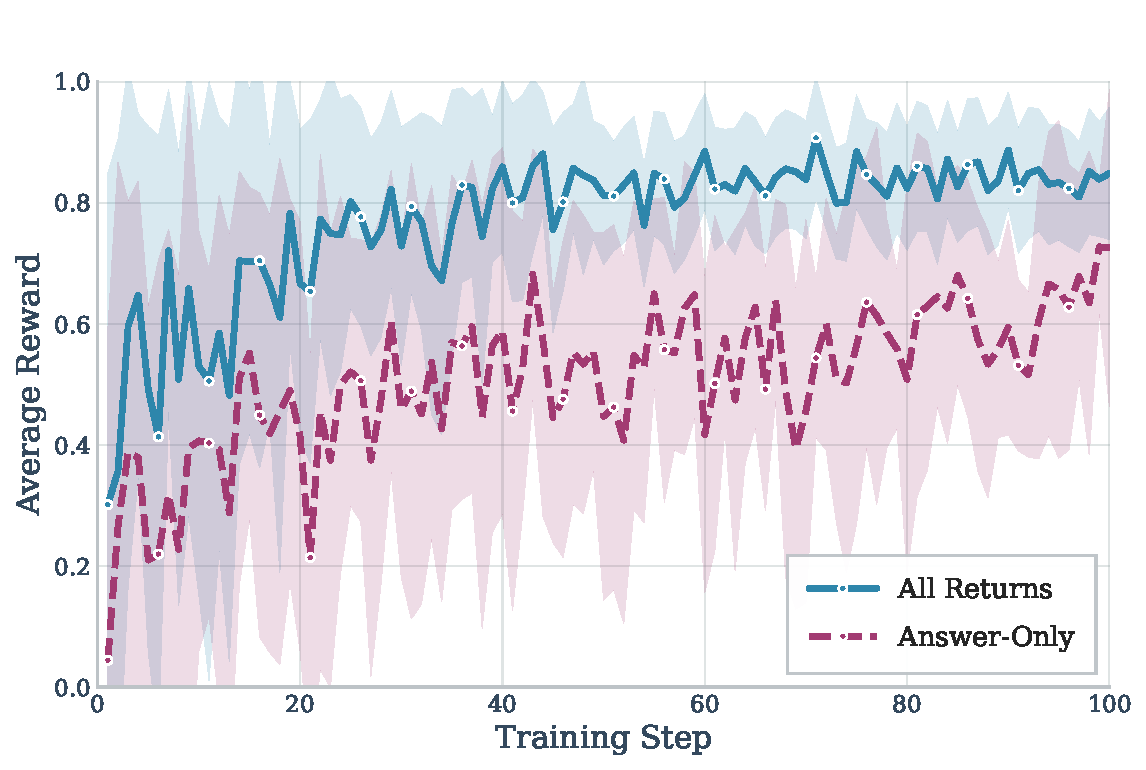
\includegraphics[width=0.8\columnwidth]{results/qwen25_7B_reward_trends.pdf}
\caption{Training convergence curves on Qwen2.5-7B-Instruct comparing All-Returns (solid line) v.s. Answer-Only (dashed line) reward strategies.}
\label{fig:reward_convergence}
\end{figure}

\begin{table}[t]
\centering
\small
\caption{Reward function ablation on HotpotQA using Qwen2.5-7B-Instruct. All-Returns v.s. Answer-Only reward strategies. ``TN'' is the token number, and ``TC'' denotes the number of tool calls.}
\label{tab:reward_ablation}
\begin{tabular}{@{}lcccc@{}}
\toprule
\textbf{Strategy} & \textbf{J}($\uparrow$) & \textbf{TN}($\downarrow$) & \textbf{MQ}($\uparrow$) & \textbf{TC}(-) \\
\midrule
Answer-Only & 0.509 & \textbf{2078} & 0.479 & 3.93 \\
All-Returns & \textbf{0.544} & 2117 & \textbf{0.533} & 4.92 \\
\bottomrule
\end{tabular}
\vspace{-0.2cm}
\end{table}

